\documentclass[11pt,a4paper]{article}
\usepackage[utf8]{inputenc}
\usepackage[brazil]{babel}
\usepackage{graphicx}
\usepackage[pdftex]{hyperref}
\usepackage[a4paper,top=3cm,bottom=2cm,left=3cm,right=3cm,marginparwidth=1.75cm]{geometry}
\title{FastFoot - Desafios de futebol online}
\author{Obede Carvalho (201410277), Gabriel Rodrigues (201321120)}
\date{}
\begin{document}

	\maketitle
	\section{Proposta}
	\section*{Objetivo do trabalho e motivação}
		O desenvolvimento do trabalho tem como objetivo um conhecimento prático por parte dos alunos das tecnologias de computação em nuvem, em especial com a arquitetura software como um serviço. Também tem como objetivo novos conhecimentos sobre tecnologias de programação, como linguagens, frameworks e padrões de desenvolvimento.

	\section*{Descrição Geral do sistema}
		O sistema será um gerenciador de times de futebol onde o usuário irá gerenciar toda a estrutura de um time de futebol, como patrocínios, negociação de jogadores, estrutura de estádio, entre outros. O usuário poderá jogar partidas de campeonatos e amistosas contra outros usuários.

	\section*{Diagrama componentes do sistema}
		O sistema estará hospedado em uma plataforma como serviços (Paas) e acessará um banco de dados também hospedado em um plataforma como serviço. O usuário acessará o sistema através de um navegador web.

	\section*{Requisitos funcionais}
		\begin{itemize}
			\item O usuário deverá criar uma conta e estar logado para acessar as funcionalidades do sistema.
			\item O usuário gerenciará todos os aspectos do time criado por ele, como nome do time, negociação de jogadores, negociação de patrocínios, estrutura do estádio, escalação do time para uma partida, escolha de formação tática.
			\item Todo time criado entrará automaticamente em um campeonato de acesso. Dentro dos campeonatos haverá promoção e rebaixamento, para outros campeonatos, para os melhores e piores times respectivamente.
			\item Os jogadores de um time terão um nível de qualidade, o que determinará o resultado dos jogos.
			\item Um time começará com jogadores de baixo nível de qualidade.
			\item Um usuário terá acesso a informações de todos os jogadores disponíveis para negociação.	
		\end{itemize}

	\section*{Requisitos não funcionais}
		\begin{itemize}
			\item O sistema deverá suportar uma grande quantidade de usuários (escalabilidade).
			\item O sistema deverá estar disponível em pelo menos 95\% do tempo.
			\item Os dados dos usuários do sistema devem estar protegidos dentro das políticas de privacidade do sistema.
		\end{itemize}

	\section*{Desafios técnicos}
		Os desafios do projeto serão com o uso de frameworks e api's necessárias para desenvolvimento da aplicação, assim como desenvolvimento de páginas web por onde o usuário acessará o sistema.
        
    \section{Projeto}
	\section*{Arquitetura do sistema}
    	O sistemas será composto de lado cliente, lado servidor e provedor de \textit{SaaS}. O lado servidor estará hospedado no provedor de \textit{SaaS} juntamente com o banco de dados da aplicação. O provedor de \textit{SaaS} será responsável por prover servidor \textit{web}, servidor de banco de dados e executar a aplicação.
    
		O usuário (lado cliente) irá requisitar páginas \textit{web} do provedor de \textit{SaaS}. Essas páginas, quando estiverem no navegador do cliente, enviaram requisições assíncronas para o servidor novamente com o intuito de receber dados e enviar modificações realizadas pelo usuário no gerenciamento de seu time.
    
	\section*{Funcionalidades}
    	As funcionalidades implementadas foram as básicas para o funcionamento do sistema:
        \begin{itemize}
        	\item Login do usuário no sistema
            \item Escolha da formação tática do time entre:
            	\begin{itemize}
                	\item 3-4-3
                    \item 3-5-2
                    \item 4-4-2
                    \item 4-3-3
                    \item 5-4-1
                \end{itemize}
           \item Escalação de jogadores
           \item Compra e venda de jogadores
           \item Marcação e rejeição de jogos amistosos
           \item Disputa de jogo amistoso:
           		\begin{itemize}
                	\item Principais lances do jogo
                    \item Resultado final do jogo
                    \item Premiação do clube vencedor
                \end{itemize}
        \end{itemize}
        As formações táticas representam o número de defensores, número de jogadores de meio-campo e número de atacantes, implicitamente há a necessidade de escalação de um goleiro, totalizando 11 jogadores.
        
        Os jogadores disponíveis podem ser Goleiro, Defensor, Meio-Campo e Atacante.
        
	\section*{Protocolos}
    	O sistema foi idealizado sobre um protocolo \textit{REST} onde a comunicação entre o servidor e o cliente são bem definidas e utilizam dados estruturados. Para isso todas as página \textit{web} deveriam fazem requisições para o servidor assincronamente (protocolo AJAX) que responderiam dados estruturados em um arquivo \textit{JSON}. Com um protocolo \textit{REST} bem definido, o sistema poderia futuramente ser acessível de outras formas, como aplicações movéis e \textit{desktop}.
        
        Na aplicação desenvolvida todas as respostas obedecem tal protocolo, exceto a página de disputa do amistoso que é montada no servidor durante os lances do amistoso e retornado assim para o usuário. Houve a necessidade de configurar o servidor para que aceitasse requisições partindo do navegor do usuário através do protocolo \textit{AJAX}, além de todas as requisições devem ser utilizando o \textit{HTTPS} (\textit{HTTP} Seguro) pois há o envio de dados.
        
	\section*{Tecnologias}
    	O sistema FastFoot foi desenvolvido na linguagem de programação \textit{PHP}, e é acessível para o usuário através de páginas \textit{web} construídas sobre a linguagem de marcação \textit{HTML}, junto com estilos \textit{CSS}. A manipulação do \textit{DOM} do \textit{HTML} e de requisições \textit{AJAX} são feitas através do \textit{framework} \textit{AngularJS}.
        
	\section*{Banco de dados}
    	O projeto de banco de dados concentrou em representar o usuário do sistema, o clube do usuário, os jogadores de um clube e os amistosos marcados. Na figura abaixo \ref{model_er} pode ser visto a relação das entidades e seus atributos.
        
        \begin{figure}[!htb]
        	\centering
        	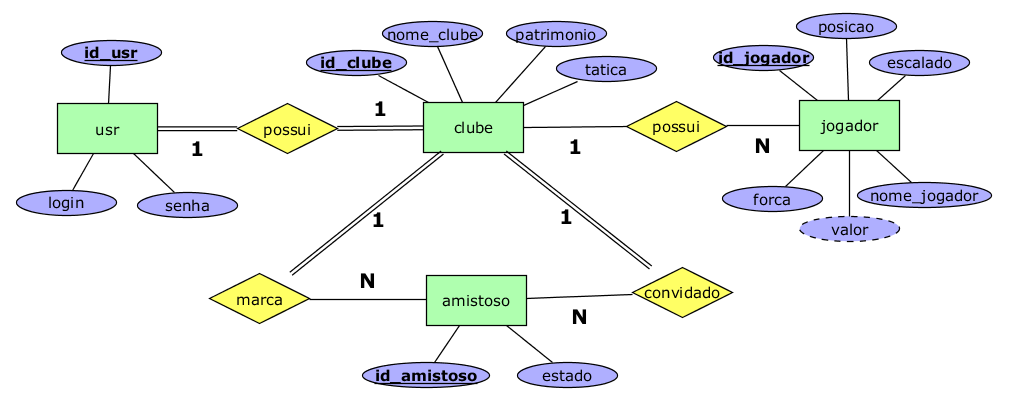
\includegraphics[scale=0.43]{fastfoot_modeloER.png}
        	\label{model_er}
            \caption{Modelo ER FastFoot}
  		\end{figure}
        
      	Um usuário (\textit{usr}) deve possuir um clube, assim como um clube deve possuir a um usuário, um clube pode ter vários jogadores e um jogador pode pertencer a um clube (jogadores sem clube são os disponíveis para a compra), um amistoso deve ser marcado por um clube e deve ter um clube convidado, um clube pode marcar e ser convidado para vários amistosos.
        
	\section*{Serviços de computacação em nuvem}
    	O sistema desenvolvido utiliza o serviço de computação em nuvem \textit{Heroku}, através do qual o usuário tem acesso ao sistema através de uma página \textit{web}. O \textit{Heroku} tem suporte para o \textit{PHP 5} que foi utilizada para desenvolver  a aplicação. 
        
        O sistema também utiliza o \textit{SGBD} Postgres, para bancos de dados relacionais, também disponível através de Heroku, onde estão armazenados todos os dados da aplicação.
        
        O FastFoot pode ser acessado através de \href{https://fastfoot.herokuapp.com/}{FastFoot}.

\end{document}